\documentclass[11pt, a4paper]{article}

% --- PACKAGES ---
\usepackage[margin=1in]{geometry}
\usepackage{amsmath}
\usepackage{graphicx}
\usepackage{xcolor}
\usepackage{float}
\usepackage{listings}
\usepackage{hyperref}
\hypersetup{colorlinks=true, linkcolor=blue, urlcolor=blue}

% --- CODE LISTING STYLE ---
\definecolor{codegreen}{rgb}{0,0.6,0}
\definecolor{codegray}{rgb}{0.5,0.5,0.5}
\definecolor{codepurple}{rgb}{0.58,0,0.82}
\definecolor{backcolour}{rgb}{0.98,0.98,0.97}
\lstdefinestyle{mystyle}{
    backgroundcolor=\color{backcolour},   
    commentstyle=\color{codegreen},
    keywordstyle=\color{blue},
    numberstyle=\tiny\color{codegray},
    stringstyle=\color{codepurple},
    basicstyle=\ttfamily\footnotesize,
    breakatwhitespace=false,         
    breaklines=true,                 
    captionpos=b,                    
    keepspaces=true,                 
    numbers=left,                    
    numbersep=5pt,                  
    showspaces=false,                
    showstringspaces=false,
    showtabs=false,                  
    tabsize=2,
    % --- ADDED LINES TO FIX OVERFULL BOXES ---
    breakautoindent=true,            % Keep indentation on broken lines
    postbreak=\mbox{\textcolor{red}{$\hookrightarrow$}\space} % Show a symbol where line broke
}
\lstset{style=mystyle}

% --- DOCUMENT START ---
\begin{document}

% --- TITLE PAGE ---
\begin{titlepage}
    \centering
    \vspace*{\fill}
    {\Huge\bfseries EE200: Signals, Systems and Networks\par}
    \vspace{1.5cm}
    {\Large\bfseries Practical Report 1: Frequency Mixer\par}
    \vspace{2cm}
    
    \large\emph{Instructor:}\\ Dr. Tushar Sandhan
    
    \vfill
    {\large \texttt{Aarav Aryaman} \\ \texttt{220012}}\par
    \vspace*{1cm}
    {\large \today\par}
\end{titlepage}

\tableofcontents
\newpage

% --- INTRODUCTION ---
\section{Introduction}
The human visual system (HVS) does not process an image uniformly; instead, it performs multi-scale analysis, instinctively separating coarse structure from fine details. This project explores this concept by treating images as 2D signals and manipulating them in the frequency domain. The core objective is to design and implement a "frequency mixer," a system that fuses two distinct images into a single, perceptually interesting hybrid. This is achieved by combining the low-frequency components of one image, which represent the overall structure and shape, with the high-frequency components of another, which represent the fine textures and edges. The final result is an image that can be perceived differently depending on viewing distance, directly demonstrating the link between spatial frequency and visual perception.

% --- THEORY AND EQUATIONS ---
\section{Governing Equations: 2D Fourier Transform}
To analyze an image's frequency content, we utilize the 2D Discrete Fourier Transform (DFT). The DFT is a mathematical tool that decomposes a signal from its original domain (in this case, the spatial domain) into its constituent frequencies. For an image, \(I(x,y)\), the spatial coordinates \((x,y)\) define the pixel locations. The DFT transforms this into a frequency domain representation, \(F(u,v)\), where \((u,v)\) represent the horizontal and vertical spatial frequencies.

\paragraph{2D Discrete Fourier Transform (DFT):}
For an N x M image \(I(x, y)\), the 2D DFT, which transforms the image from the spatial domain to the frequency domain, is defined as:
\begin{equation}
    F(u, v) = \sum_{x=0}^{N-1} \sum_{y=0}^{M-1} I(x, y) e^{-j2\pi(\frac{ux}{N} + \frac{vy}{M})}
\end{equation}
where \(F(u, v)\) is the complex value of the frequency component \((u, v)\).
This equation calculates the presence and phase of each frequency component \((u,v)\) within the original image \(I(x,y)\).

\paragraph{2D Inverse DFT (IDFT):}
To reconstruct the image from its frequency representation, the Inverse DFT is used:
\begin{equation}
    I(x, y) = \frac{1}{NM} \sum_{u=0}^{N-1} \sum_{v=0}^{M-1} F(u, v) e^{j2\pi(\frac{ux}{N} + \frac{vy}{M})}
\end{equation}
This equation reconstructs the original image by summing all its frequency components, each weighted by its complex magnitude from \(F(u,v)\).

% --- IMAGE ANALYSIS ---
\section{Analysis of an Input Image}
An initial analysis was performed on a single input image (the dog) to understand its spectral properties.

\subsection{Spectrum Analysis and Centering}
The 2D DFT of the image was calculated and its magnitude spectrum was plotted in normal (log scaled for visibility) and decibel (dB) form, as shown in Figure \ref{fig:spectra}.

\paragraph{Spectrum Centering:} The raw output of the DFT algorithm places the zero-frequency component (DC value), which represents the average brightness of the entire image, at the \textbf{top-left corner (index [0,0])}. As a result, the other low-frequency components are located at the four corners of the spectrum image, which is not intuitive for analysis. To correct this, the \texttt{scipy.fft.fftshift} function was used. This function swaps the quadrants of the spectrum, moving the \textbf{low frequencies to the center and the high frequencies to the outer regions}. This centered representation is standard practice, as it provides a clear visual map where the bright central area corresponds to the dominant, low-frequency structural components of the image, and the dimmer outer areas correspond to the high-frequency details and edges.

\begin{figure}[H]
    \centering
    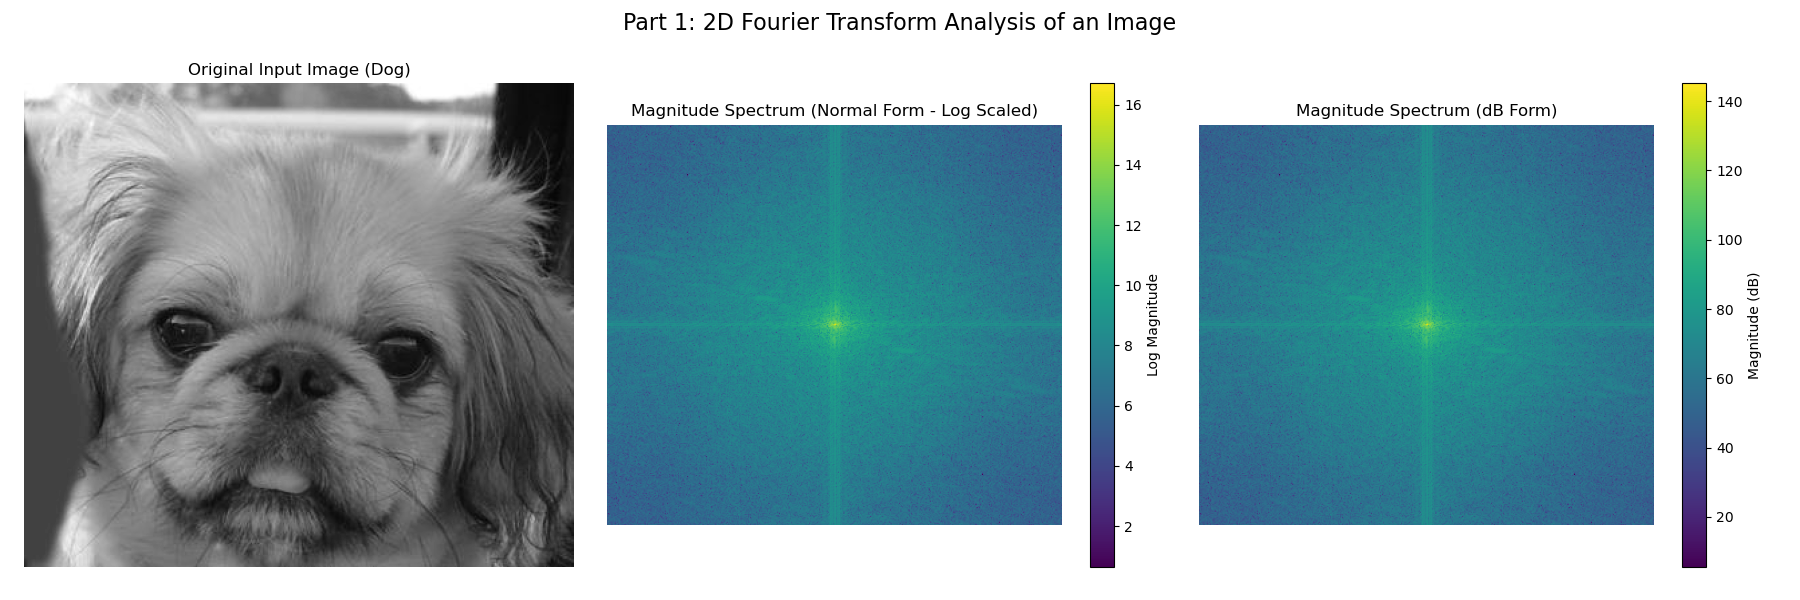
\includegraphics[width=\textwidth]{q1_part1_spectra_analysis.png}
    \caption{Analysis of the dog image's Fourier magnitude spectrum.}
    \label{fig:spectra}
\end{figure}

\subsection{Effect of Image Rotation}
The input image was rotated 90 degrees anticlockwise to observe the corresponding effect in the frequency domain.

\begin{figure}[H]
    \centering
    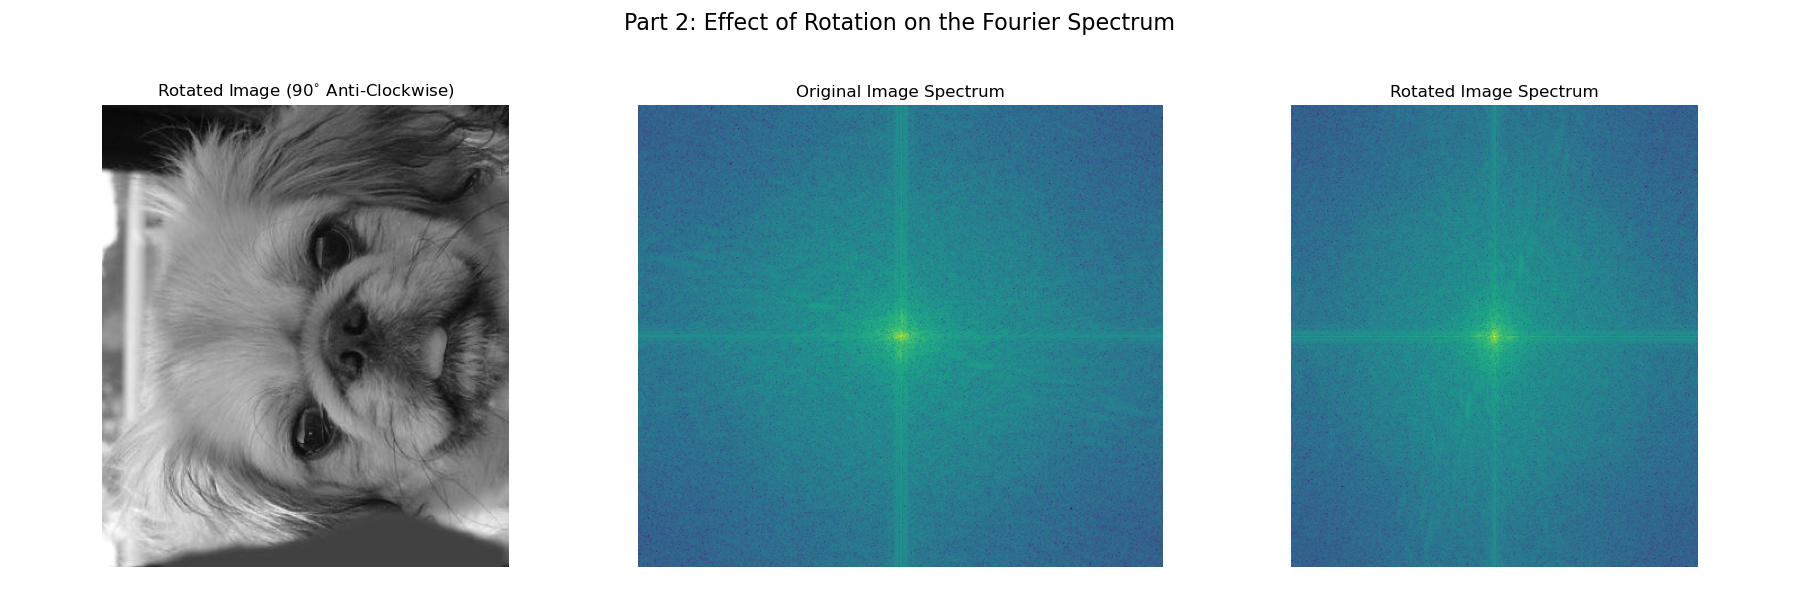
\includegraphics[width=\textwidth]{q1_part2_rotation_analysis.png}
    \caption{Comparison of the original spectrum and the spectrum of the rotated image.}
    \label{fig:rotation}
\end{figure}

\paragraph{Observation:} As demonstrated in Figure \ref{fig:rotation}, a 90 degree rotation of the image in the spatial domain results in an identical 90-degree rotation of its magnitude spectrum in the frequency domain. This result visually confirms the \textbf{rotation property of the 2D Fourier Transform}, where a rotation in the spatial domain corresponds directly to an equivalent rotation in the frequency domain.

% --- FREQUENCY MIXER ---
\section{The Frequency Mixer System}
A system was designed to fuse the two input images. The low-frequency structural information from the dog image was combined with the high-frequency detail information from the cat image.

\subsection{System Design and Transfer Functions}
The system operates by filtering each image in the frequency domain. These filters act as the system's \textbf{transfer functions}, dictating which frequencies are passed and which are attenuated for each input signal. A specific cutoff frequency of 13 was chosen as the primary design parameter, as it produced a visually effective and compelling hybrid illusion.

\begin{enumerate}
    \item \textbf{Low-Pass Filter (LPF):} A \textbf{Gaussian} LPF was designed to isolate the low frequencies from the dog image. A Gaussian function was specifically chosen because it is smooth and has no sharp edges. This property is crucial as it prevents the introduction of "ringing" artifacts (Gibbs phenomenon) in the reconstructed image, which would occur with an ideal, sharp-edged filter. Its transfer function, \(H_{low}(u, v)\), is shown in Figure \ref{fig:overview}.
    
    \item \textbf{High-Pass Filter (HPF):} A corresponding HPF was created by subtracting the Gaussian LPF from an all-pass filter: \(H_{high}(u, v) = 1 - H_{low}(u, v)\). This complementary filter was used to extract the fine details from the cat image by attenuating its low-frequency components.
\end{enumerate}

Figure \ref{fig:overview} provides a detailed plot of this designed system, showing the inputs, the transfer functions, and the resulting filtered images.

\begin{figure}[H]
    \centering
    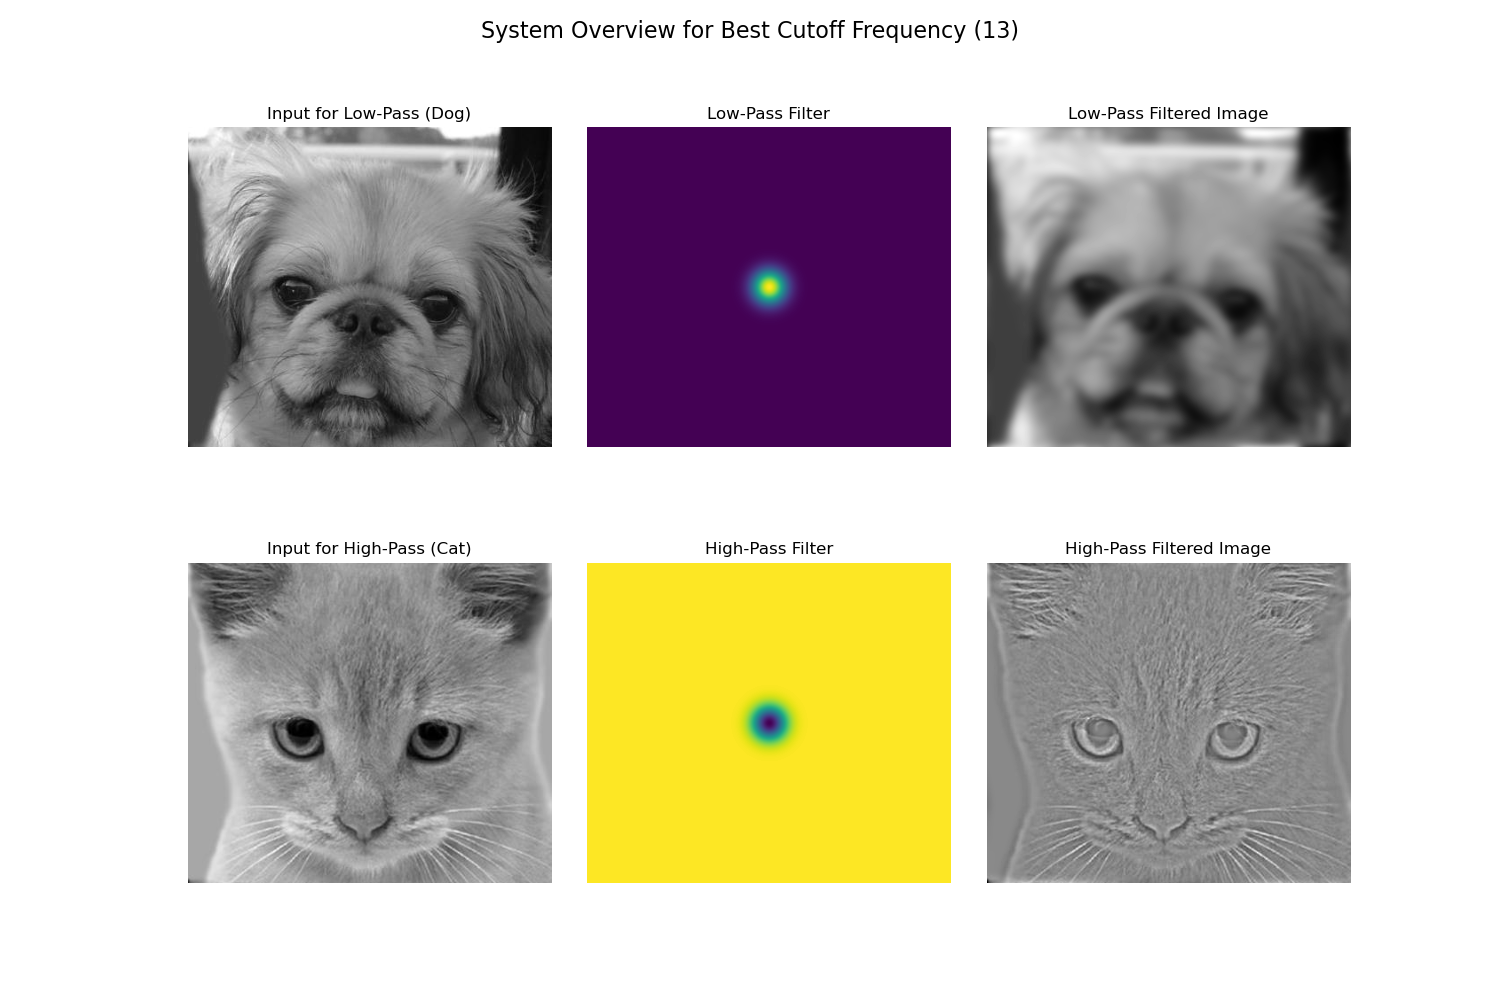
\includegraphics[width=\textwidth]{q1_part3_system_overview.png}
    \caption{Detailed overview of the frequency mixer system for the chosen cutoff frequency of 15. Top Row: The low-pass path. Bottom Row: The high-pass path.}
    \label{fig:overview}
\end{figure}

\subsection{Final Result and Component Visualization}
The final hybrid image is a linear summation of the low-pass filtered dog image and the high-pass filtered cat image in the frequency domain. To demonstrate how the illusion works at different perceptual scales, Figure \ref{fig:composite} was created. It shows the final hybrid image alongside its constituent low-pass and high-pass components generated at four different frequency cutoffs.

\begin{figure}[H]
    \centering
    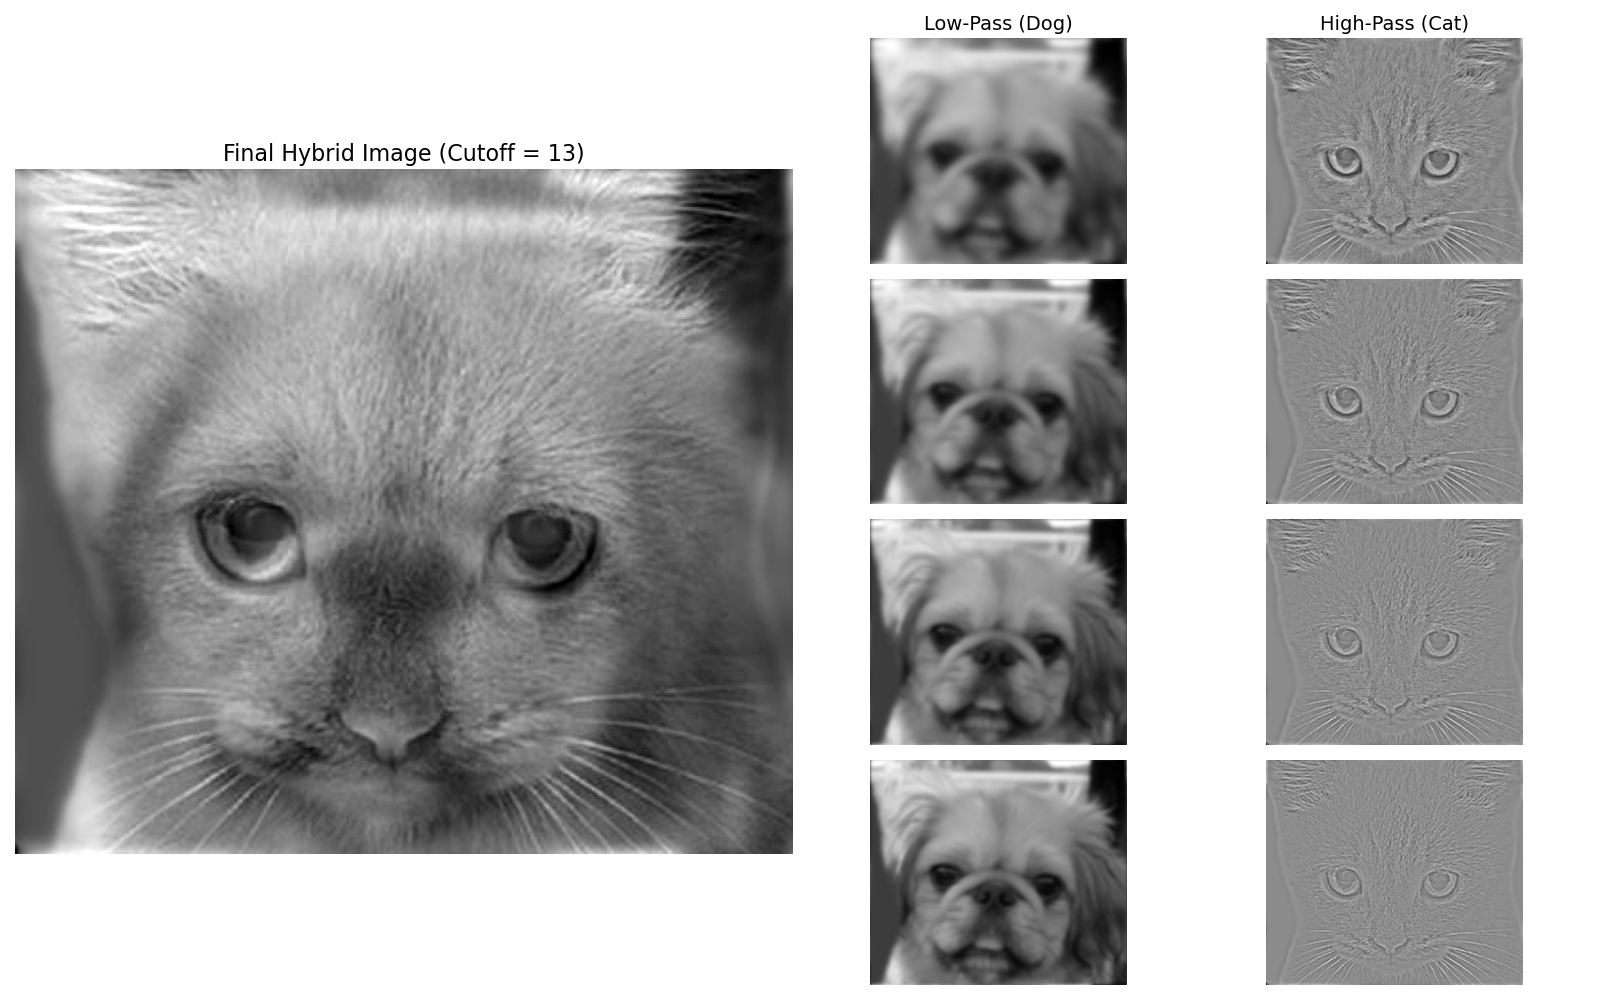
\includegraphics[width=\textwidth]{q1_part3_composite_visualization.png}
    \caption{Final composite visualization. The main hybrid image (left) is shown alongside its low-pass (Dog) and high-pass (Cat) components at varying frequency cutoffs (right).}
    \label{fig:composite}
\end{figure}

This visualization powerfully illustrates the core concept: when an observer is far away (or squints), their visual system naturally performs a low-pass filtering operation. This blurs out the high-frequency details of the cat, causing the low-frequency structure of the dog to dominate perception. Conversely, when viewed up close, the high-frequency details of the cat's face become salient and easily discernible, overriding the blurry, low-frequency background. The grid on the right side of Figure \ref{fig:composite} explicitly shows these separated components, making it clear how the final image is constructed and why the perceptual effect occurs.

% --- CONCLUSION ---
\section{Conclusion}
This project successfully demonstrated the use of the 2D Fourier Transform for image analysis and manipulation. The properties of the Fourier spectrum, including its centering and response to rotation, were verified. A frequency mixer system was designed and implemented that successfully fused two images by combining their respective low and high spatial frequencies. The final visualizations effectively illustrate the system's mechanics and the perceptual basis of the hybrid image illusion.

% --- APPENDIX ---
\appendix
\section{Final Python Code}
\begin{lstlisting}[language=Python, caption={Python script for Question 1.}]
# ============================================================================
# EE200: Signals, Systems and Networks
# Code for Question 1: Frequency Mixer
# ============================================================================

# ============================================================================
# --- CONFIGURATION AND SETUP ---
# ============================================================================

import numpy as np
import matplotlib.pyplot as plt
from PIL import Image
from scipy.fft import fft2, fftshift, ifft2, ifftshift
from matplotlib.gridspec import GridSpec
import os

# Input file paths
IMAGE_CAT_PATH = 'cat_gray.jpg'
IMAGE_DOG_PATH = 'dog_gray.jpg'

# Output directory for all generated files
OUTPUT_DIR = 'q1_final_submission_outputs'

# --- Parameters for the Hybrid Image ---
# The cutoff frequency that produces the best visual illusion for the main hybrid image.
BEST_HYBRID_CUTOFF = 13

# To demonstrate the effect of changing the filter parameters.
GRID_CUTOFF_FREQUENCIES = [10, 15, 20, 25]

# Create the output directory
os.makedirs(OUTPUT_DIR, exist_ok=True)
print(f"All outputs for Question 1 will be saved in: '{OUTPUT_DIR}/'")

# ============================================================================
# --- PART 1: 2D FOURIER TRANSFORM OF A SINGLE IMAGE ---
# ============================================================================

print("\nPART 1: Analyzing the 2D Fourier Transform of a Single Image...")

try:
    # We'll use the dog image for this initial analysis
    img_single_pil = Image.open(IMAGE_DOG_PATH).convert('L')
except FileNotFoundError:
    print(f"Error: '{IMAGE_DOG_PATH}' not found. Please check the file path.")
    # Fallback to a dummy image to prevent script crash
    img_single_pil = Image.fromarray(np.random.randint(0, 255, (400, 400), dtype=np.uint8))

img_single_array = np.array(img_single_pil, dtype=float)
F_single_shifted = fftshift(fft2(img_single_array))

# Calculate spectra in normal and dB forms
magnitude_spectrum_normal = np.abs(F_single_shifted)
magnitude_spectrum_db = 20 * np.log10(magnitude_spectrum_normal + 1)

# Create and save the analysis plot
fig1, axes1 = plt.subplots(1, 3, figsize=(18, 6))
fig1.suptitle('Part 1: 2D Fourier Transform Analysis of an Image', fontsize=16)

axes1[0].imshow(img_single_array, cmap='gray'); 
axes1[0].set_title('Original Input Image (Dog)'); 
axes1[0].axis('off')

im1 = axes1[1].imshow(np.log(magnitude_spectrum_normal + 1), cmap='viridis'); 
axes1[1].set_title('Magnitude Spectrum (Normal Form - Log Scaled)'); 
axes1[1].axis('off'); fig1.colorbar(im1, ax=axes1[1], label='Log Magnitude')

im2 = axes1[2].imshow(magnitude_spectrum_db, cmap='viridis'); 
axes1[2].set_title('Magnitude Spectrum (dB Form)'); 
axes1[2].axis('off'); fig1.colorbar(im2, ax=axes1[2], label='Magnitude (dB)')

fig1.tight_layout(rect=[0, 0.03, 1, 0.95])
plt.savefig(os.path.join(OUTPUT_DIR, 'q1_part1_spectra_analysis.png'))
plt.show()

# ============================================================================
# --- PART 2: ROTATION ANALYSIS ---
# ============================================================================

print("\nPART 2: Analyzing the Effect of Rotation on the Fourier Spectrum...")

img_rotated = img_single_pil.rotate(90, expand=True)
img_rotated_array = np.array(img_rotated, dtype=float)
magnitude_spectrum_rotated = np.log(np.abs(fftshift(fft2(img_rotated_array))) + 1)

# Create and save the rotation analysis plot
fig2, axes2 = plt.subplots(1, 3, figsize=(18, 6))
fig2.suptitle('Part 2: Effect of Rotation on the Fourier Spectrum', fontsize=16)

axes2[0].imshow(img_rotated_array, cmap='gray'); 
axes2[0].set_title('Rotated Image (90$^{\circ}$ Anti-Clockwise)'); 
axes2[0].axis('off')

axes2[1].imshow(np.log(magnitude_spectrum_normal + 1), cmap='viridis'); 
axes2[1].set_title('Original Image Spectrum'); 
axes2[1].axis('off')

axes2[2].imshow(magnitude_spectrum_rotated, cmap='viridis'); 
axes2[2].set_title('Rotated Image Spectrum'); 
axes2[2].axis('off')

fig2.tight_layout(rect=[0, 0.03, 1, 0.95])
plt.savefig(os.path.join(OUTPUT_DIR, 'q1_part2_rotation_analysis.png'))
plt.show()

# ============================================================================
# --- PART 3: CREATIVE FUSION (CAT-HIGH, DOG-LOW) ---
# ============================================================================

print("\nPART 3: Creating and Visualizing the Hybrid Image...")

try:
    img_high_pil = Image.open(IMAGE_CAT_PATH).convert('L') # Cat provides high frequencies
    img_low_pil = Image.open(IMAGE_DOG_PATH).convert('L')  # Dog provides low frequencies
except FileNotFoundError: exit("Error: Could not find Cat or Dog image. Aborting.")

if img_high_pil.size != img_low_pil.size: img_high_pil = img_high_pil.resize(img_low_pil.size)

arr_high = np.array(img_high_pil, dtype=float); arr_low = np.array(img_low_pil, dtype=float)
F_high_shifted = fftshift(fft2(arr_high)); F_low_shifted = fftshift(fft2(arr_low))

# --- A) Generate components for the multi-level grid visualization ---
low_pass_components, high_pass_components = [], []
print("--> Generating component images for the multi-level grid...")
for cutoff in GRID_CUTOFF_FREQUENCIES:
    rows, cols = arr_low.shape; crow, ccol = rows // 2, cols // 2
    x, y = np.meshgrid(np.arange(cols), np.arange(rows)); dist = np.sqrt((x - ccol)**2 + (y - crow)**2)
    lpf = np.exp(-(dist**2) / (2 * cutoff**2)); hpf = 1.0 - lpf
    F_low_f = F_low_shifted * lpf; F_high_f = F_high_shifted * hpf
    low_pass_components.append(np.clip(np.real(ifft2(ifftshift(F_low_f))), 0, 255))
    high_pass_components.append(np.clip(np.real(ifft2(ifftshift(F_high_f))) + 128, 0, 255))

# --- B) Create the final hybrid and the detailed system overview for the BEST cutoff ---
print(f"--> Creating final hybrid and detailed system overview for chosen cutoff = {BEST_HYBRID_CUTOFF}...")
rows, cols = arr_low.shape; crow, ccol = rows // 2, cols // 2
x, y = np.meshgrid(np.arange(cols), np.arange(rows)); dist = np.sqrt((x - ccol)**2 + (y - crow)**2)
final_lpf = np.exp(-(dist**2) / (2 * BEST_HYBRID_CUTOFF**2)); final_hpf = 1.0 - final_lpf

F_final_low = F_low_shifted * final_lpf; F_final_high = F_high_shifted * final_hpf
F_final_hybrid = F_final_low + F_final_high
final_hybrid_image = np.clip(np.real(ifft2(ifftshift(F_final_hybrid))), 0, 255)
Image.fromarray(final_hybrid_image.astype(np.uint8)).save(os.path.join(OUTPUT_DIR, 'Cat-Dog_Hybrid_Final.png'))

final_low_pass_img = np.clip(np.real(ifft2(ifftshift(F_final_low))), 0, 255)
final_high_pass_display_img = np.clip(np.real(ifft2(ifftshift(F_final_high))) + 128, 0, 255)

# --- Plot A: The Detailed System Overview for Best Cutoff ---
fig_overview, axes_overview = plt.subplots(2, 3, figsize=(15, 10))
fig_overview.suptitle(f'System Overview for Best Cutoff Frequency ({BEST_HYBRID_CUTOFF})', fontsize=16)

axes_overview[0, 0].imshow(arr_low, cmap='gray'); 
axes_overview[0, 0].set_title('Input for Low-Pass (Dog)');

axes_overview[0, 1].imshow(final_lpf, cmap='viridis'); \
axes_overview[0, 1].set_title('Low-Pass Filter');

axes_overview[0, 2].imshow(final_low_pass_img, cmap='gray'); 
axes_overview[0, 2].set_title('Low-Pass Filtered Image');

axes_overview[1, 0].imshow(arr_high, cmap='gray'); 
axes_overview[1, 0].set_title('Input for High-Pass (Cat)');

axes_overview[1, 1].imshow(final_hpf, cmap='viridis'); 
axes_overview[1, 1].set_title('High-Pass Filter');

axes_overview[1, 2].imshow(final_high_pass_display_img, cmap='gray'); 
axes_overview[1, 2].set_title('High-Pass Filtered Image');

for ax in axes_overview.flat: ax.axis('off')

fig_overview.subplots_adjust(hspace=0.3, wspace=0.1) 
plt.savefig(os.path.join(OUTPUT_DIR, 'q1_part3_system_overview.png'))
plt.show()

# --- Plot B: The Final Composite Visualization ---
print("--> Assembling the final composite visualization figure...")
fig_composite = plt.figure(figsize=(16, 10))
gs = GridSpec(len(GRID_CUTOFF_FREQUENCIES), 4, figure=fig_composite)

ax_main = fig_composite.add_subplot(gs[:, 0:2]); 
ax_main.imshow(final_hybrid_image, cmap='gray');
ax_main.set_title(f'Final Hybrid Image (Cutoff = {BEST_HYBRID_CUTOFF})', fontsize=16); 
ax_main.axis('off')

for i in range(len(GRID_CUTOFF_FREQUENCIES)):
    ax_lp = fig_composite.add_subplot(gs[i, 2]); ax_lp.imshow(low_pass_components[i], cmap='gray'); ax_lp.axis('off')
    if i == 0: ax_lp.set_title('Low-Pass (Dog)', fontsize=14)
    ax_hp = fig_composite.add_subplot(gs[i, 3]); ax_hp.imshow(high_pass_components[i], cmap='gray'); ax_hp.axis('off')
    if i == 0: ax_hp.set_title('High-Pass (Cat)', fontsize=14)

fig_composite.tight_layout()
plt.savefig(os.path.join(OUTPUT_DIR, 'q1_part3_composite_visualization.png'))
plt.show()

# ============================================================================
# --- END ---
# ============================================================================

\end{lstlisting}

\end{document}